% =========================================================
% CONFIGURACION DEL DOCUMENTO
% =========================================================
\providecommand{\main}{..}
\documentclass[../main.tex]{subfiles}

% =========================================================
% CONTENIDO
% =========================================================
\begin{document}		
\chapter{Estado del arte}
\label{cha:02_estado_del_arte}

	En base a la investigación previa fue posible definir de forma genérica los elementos principales requeridos para la configuración y puesta en marcha de un sistema de estimulación visual y registro de movimiento ocular. De esta forma se presenta a continuación un diagrama general de funcionamiento del sistema final y una imagen de ejemplo de un setup típico implementado:   

	\begin{figure}[H]
		\centering
		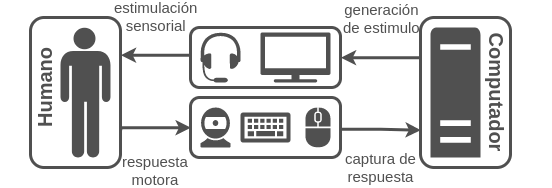
\includegraphics[width=0.7\textwidth]{cap_02_diagram}
		\caption{Diagrama general de la interfaz hombre-máquina \cite{website:baseInfo}.}
		\label{fig:02_diagrama_interfaz}
	\end{figure}

	En esta figura se pretende explicitar la función del sistema de estimulación - adquisición - registro y los requerimientos del mismo. Así, el software asociado debe ser capaz de manejar la interfaz con el usuario para poder entregar estímulos (visuales principalmente) y recibir las respuestas asociadas (en forma de datos de posicionamiento ocular o respuestas solicitadas por pantalla) de forma tal de agrupar las acciones temporalmente permitiendo de esta forma dar sentido a los datos obtenidos en el experimento. 

	\newpage
	De esta forma, una implementación típica sería como se muestra a continuación:  

	\begin{figure}[H]
		\centering
		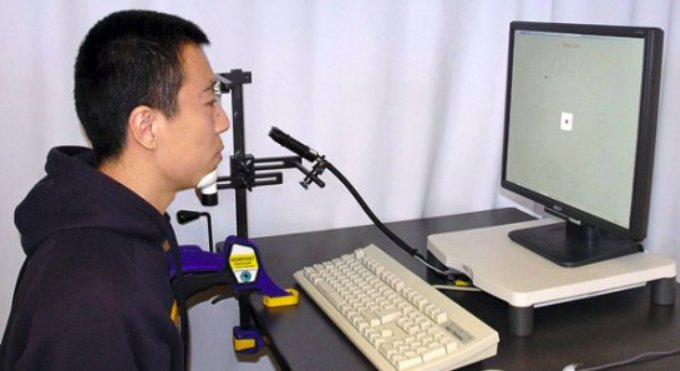
\includegraphics[width=0.5\textwidth]{cap_02_setup}
		\caption{Setup experimental típico \cite{website:baseInfo}.}
		\label{fig:02_ejemplo_setup}
	\end{figure}

	Para comprender de mejor manera el sistema y sus componentes, se presentará a modo de introducción en este capítulo una descripción de los elementos principales que forman parte del mismo. 

	\section{Sistemas de seguimiento ocular}
	\label{sec:02_sistemas_de_seguimiento_ocular}
		\subsection{Movimiento ocular}
		\label{sub:02_movimiento_ocular}

		La acción de dirigir la mirada hacia un objeto es parte fundamental del proceso de visión. Este acto involucra el direccionamiento de los ejes visuales\footnote{Corresponde a la proyección de una línea recta que pasa simultáneamente por el centro de la fóvea, área de la retina que permite la visión más nítida y detallada, y la pupila.} hacia un objetivo determinado, permitiendo la realización de análisis visuales precisos. Dicha orientación muchas veces implica movimientos coordinados de los ojos, cuello y cabeza, no obstante, existen movimientos más pequeños que son realizados únicamente por los ojos, conocidos como movimientos sacádicos \cite{article:movOcular, website:movOcular}.

		Los movimientos sacádicos corresponden a las rotaciones que realiza el globo ocular entre dos momentos de posicionamiento estacionario y que se traducen en el desplazamiento de la pupila. Estos desplazamientos pueden ocurrir tanto en el eje horizontal como vertical y cabe destacar que durante los periodos de tiempo en que se realiza el movimiento los ojos no entregan información visual relevante. Para individuos en condiciones normales este tipo de movimiento se realiza constantemente y se repite varias veces por segundo, el direccionamiento de los ojos en estos casos suele ser controlado por procesos cognitivos realizados de forma inconsciente.

		Las características principales de dichos movimientos son:
		\begin{enumerate}
			\item Cada sacada tiene un patrón de movimiento similar, por lo tanto son altamente caracterizables.

			\item Por su naturaleza los movimientos sacádicos son denominados balísticos, esto quiere decir que la posición de destino se encuentra predeterminada en el momento de partida. 

			\item La velocidad de las sacadas aumenta de forma no lineal en la medida que aumenta la amplitud de movimento (cosa que se cumple bajo toda circunstancia). De esta forma la duración del movimiento puede fluctuar entre $20 - 100[ms]$ y sus velocidades entre $10 - 300 [\frac{deg}{s}]$.

			\item La precisión de la sacada fluctúa entre un $5-10\%$ de la amplitud total del movimiento y las correcciones son realizadas por desplazamientos de calibración denominados micro-sacadas. Estos métodos correctivos permiten suponer que existe algún tipo de procesamiento paralelo encargado de la calibración ocular de largo plazo \cite{website:movOcular}.  

		\end{enumerate}

		Las características expuestas entregan, a grandes razgos, nociones que permiten comprender el por qué su estudio se ha vuelto común en campos científicos como la neurociencia: Dado que los movimientos del globo ocular son caracterizables, de patrones definidos y de alta presición es posible identificar mediante ellos enfermedades cuyos síntomas se traduzcan en alteraciones de las capacidades motrices. Un ejemplo de esto es la enfermedad de Parkinson, donde una afección crónica a los ganglios basales produce una reducción progresiva de la sustancia negra lo que se traduce en una producción insuficiente de dopamina, neurotransmisor relevante para la función motora. Esta insuficiencia se traduce en aumentos en los tiempos de respuesta y tasas de error en diversas tareas asociadas a movimiento ocular (ver \ref{sub:02_experimentos_de_estimulacion}).    

		\subsection{Métodos de captura}
		\label{sub:02_metodos_de_captura}
			\subsubsection{Un poco de historia} 
			\label{ssub:02_un_poco_de_historia_monitores}
			
			Para poder registrar los movimientos oculares es necesario el uso de equipamiento especializado y que, por su funcion y sin importar la tecnología utilizada, se denomina por su nombre en inglés: eye tracker. A modo introductorio se presenta a continuación una pincelada de su desarrollo en la historia \cite{article:eyetracker_eggert, article:eyetracker_richardson}

			La primera aparición de dispositivos de este tipo data de finales del siglo XIX (Delabarre y Hale). Sus primeras versiones consistian en sistemas sumamente invasivos donde alambres finos conectados a una especie de lente de contacto movían una serie de palancas que amplificaban el movimiento y lo registraban en papel. Este método permitió objetivizar las investigaciones de comportamiento existentes. Por su contrucción, dichos dispositivos permitían observar el comportamiento espacial, más no el temporal. 

			A principios del siglo XX y de la mano de técnicas no invasivas basadas en óptica y reflexión de luz comenzaron a desarrollarse sistemas más parecidos a las tecnologías actuales: La proyección de luz sobre la córnea genera reflejos que se mueven de forma similar a la pupila y por tanto si se hace posible su registro, es posible conocer el movimiento ocular tanto horizontal como vertical, más no rotatorio (Dodge y Cline). Este método revolucionario marcaría los desarrollos futuros en esta área.

			En la década de los 70' y gracias con los avances en sistemas de grabación de video y procesamiento digital se hizo posible detectar electrónicamente características del movimiento en base al contraste existente entre la esclerótida\footnote{Sección blanca del ojo que rodea a la pupila} y los bordes del iris. Debido a los efectos de sombra producidos por los párpados este método presentaba problemas para detectar movimientos verticales, no obstante, permitía registrar movimiento horizontal con buena calidad. 

			De forma posterior y en base a estos avances iniciales fueron desarrolladas las tecnologías que, cada vez más, permiten obtener información relevante sin producir daño sobre quienes forman parte de los experimentos, reduciendo así las limitantes en este campo de investigación.    

			\subsubsection{Tecnologías actuales}
			\label{ssub:02_tecnologias_actuales}

				En la actualidad existen una gran gama de tecnologías para registrar movimiento ocular \cite{article:eyetracker_eggert, article:eyetracker_richardson, dissertation:eyetrackers}, no obstante, a continuación se muestran mas relevantes y utilizadas: 
				\begin{enumerate}
					\item \textbf{Bobina escleral magnética (SSG):} Esta técnica requiere del uso de lentes de contacto de gran tamaño directamente sobre el globo ocular. Dicho lente posee dos pequeñas bobinas de alambre que, al ser alineadas con el eje de visión, permiten obtener información sobre la dirección en la que se encuentra el ojo en forma de voltaje al ser inducidas por campos electromagnéticos externos de alta frecuencia. A pesar de la gran incomodidad que producen, esta técnica es una de las más precisas y exactas.
					\begin{figure}[H]
						\centering
						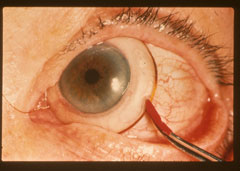
\includegraphics[width=0.35\textwidth]{cap_02_et_ssg}
						\caption{Ejemplo de uso de SSG \cite{website:etSSG}.}
						\label{fig:02_et_ssg}
					\end{figure}

					\item \textbf{Electro-OculoGrafía (EOG):} Esta técnica de seguimiento ocular se basa en la medición de diferencias de potencial eléctrico en la piel que se encuentra al rededor del ojo. En la medida que el ojo rota, el dipolo producido por la córnea y la retina cambia, lo que se ve reflejado en las mediciones. Sus ventajas principales, además del bajo costo, son la capacidad de medir movimiento ocular a pesar de que los ojos se encuentren cerrados, lo que hace de este método una herramienta interesante en caso de estudio de sueño y que las mediciones son relativas a la posición de la cabeza. No obstante lo anterior, la precisión y exactitud de las mediciones obtenidas es baja ya que se encuentran sujetas a artefactos como el movimiento de los párpados.
					\begin{figure}[H]
						\centering
						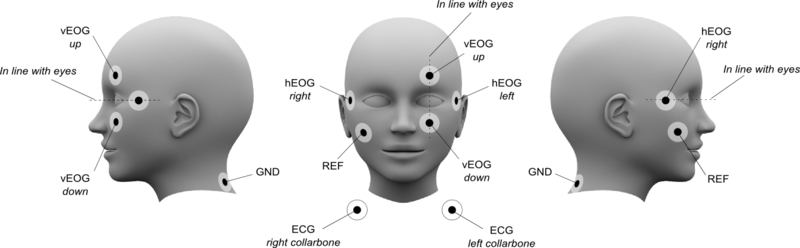
\includegraphics[width=0.9\textwidth]{cap_02_et_eog}
						\caption{Ejemplo de posicionamiento de electrodos para EOG \cite{website:etEOG}.}
						\label{fig:02_et_eog}
					\end{figure}

					\item \textbf{Seguimiento ocular basado en video (VOG):} Este tipo de tecnología es la más utilizada en la actualidad y corresponde a la grabación y procesamiento de la información recibida de una o más cámaras. El procesamiento puede ser dividido en dos etapas principales: en la primera se detecta y localiza el ojo en la imagen, para lo que típicamente se utiliza la pupila o el iris como punto de referencia y la segunda etapa corresponde al proceso por el cual se estima hacia donde se dirige la mirada. 

					Dentro de las técnicas VOG existentes la más popular corresponde a la detección de reflexiones de luz en la pupila y córnea. Este método suele emplear una o más cámaras y focos de luz, típicamente de tecnología infrarroja, ubicados cerca de la fuente de estimulación visual y orientados hacia el globo ocular. La tecnología infrarroja permite producir reflexiones de luz sin provocar molestia en el usuario, además de lograr evitar la mayor parte de contaminación lumínica externa. 

					El principio de funcionamiento de los métodos de reflexión se basa en las imagenes de Purkinje-Sanson que describen la existencia de al menos 4 reflexiones de luz que pueden ser utilizadas como referencia para estimar el direccionamiento de la pupila. Además, los precios de los dispositivos que utilizan esta técnica suelen encontrarse relacionados a la cantidad o tipo de reflexiones utilizadas.
					\begin{figure}[H]
						\centering
						\subfloat[Reflexiones de Purkije-Sanson]{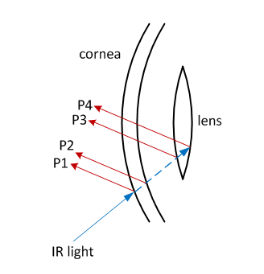
\includegraphics[width=0.25\textwidth]{cap_02_et_vog1}}\hspace{5mm}
						\subfloat[Posición de las reflexiones de la córnea (P1) relativas al centro de la pupila.]{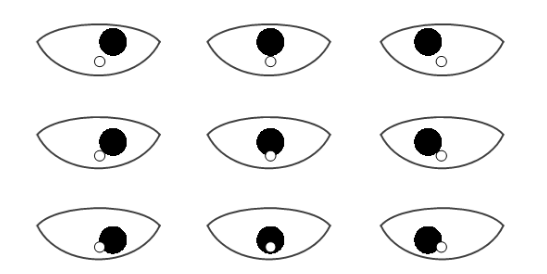
\includegraphics[width=0.55\textwidth]{cap_02_et_vog2}}
						\caption{Principio de detección VOG en base a reflexión de luz\cite{dissertation:eyetrackers}.}
						\label{fig:02_et_vog1}
					\end{figure}

					La presentación de estos dispositivos es variada y van desde cascos y lentes hasta trípodes y columnas donde se integran un elemento apoya-baribilla y el eye tracker. A continuación se muestran algunos a modo de referencia:
					\begin{figure}[H]
						\centering
						\subfloat[Tobii Pro Glasses 2 \cite{website:tobii}]{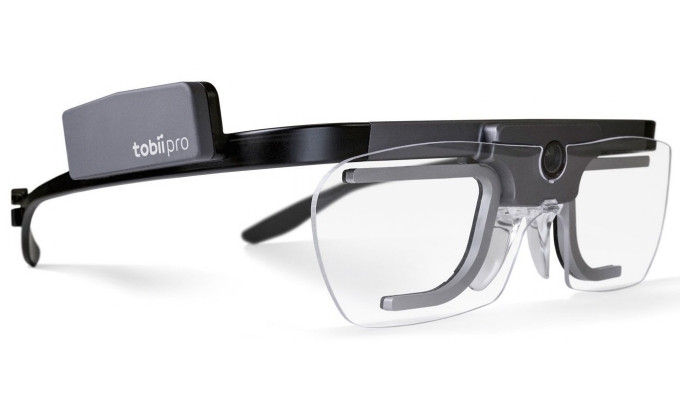
\includegraphics[width=0.4\textwidth]{cap_02_et_vog_1}}\hspace{5mm}
						\subfloat[MiraMetrix S2 \cite{website:microway}]{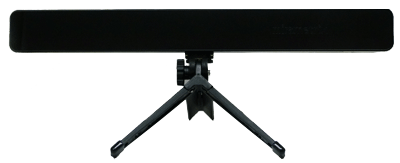
\includegraphics[width=0.4\textwidth]{cap_02_et_vog_2}}
						\caption{Muestra de eyetrackers disponibles en el mercado.}
						\label{fig:02_et_vog2}
					\end{figure}  

				\end{enumerate}

			\subsubsection{Comparativa}
			\label{ssub:02_comparativa_eyetracker}

			a pesar de las claras e importantes diferencias entre las tecnologías presentadas es posible realizar una comparación entre las mismas. En \cite{article:eyetracker_eggert, article:eyetracker_richardson, dissertation:eyetrackers} se entregan nociones sobre las capacidades operativas en cuanto a presición espacial, temporal, capacidad de registrar movimientos de torsión, desplazamiento horizontal y vertical, tiempo requerido para preparar su uso (setup), comodidad para el usuario tipo de calibración requerida y complejidad de la misma. 

			A continuación se presenta una tabla resumen con las características ya descritas para EOG, SSG, VOG (común) y DPI (VOG de gama alta utilizando distintas reflexiones de Purkinje): 
			
			\begin{table}[H]\begin{center}\fontsize{8pt}{1em}{
				\singlespacing{\begin{tabular}{| C{0.18\textwidth} | C{0.18\textwidth} | C{0.18\textwidth} | C{0.18\textwidth} | C{0.18\textwidth}|}
					\hline
					 & EOG & SSG & VOG & DPI \\ \hline
					Precisión espacial (grados)	& $\approx 0.5$ & $\approx 0.01$ & $\approx 0.05$ & $\approx 0.017$\\ \hline
					Precisión temporal (Hz) 	& $40$ & $500$ & $50-400$ & $500-1000$\\ \hline
					Registro de mov. verticales	& Es posible pero se encuentran sujetos a error por efecto de artefactos producidos por el párpado & Si & Si & Si \\ \hline
					Registro de torsión			& No & Si & Si & Si \\ \hline
					Tiempo de setup				& Lento debido a que requiere la utilización de electrodos & Lento & Rápido & Rápido \\ \hline
					Requiere calibración por enfoque & Si & No & Si & Si \\ \hline
					Complejidad de calibración	& Requiere configuración bitemporal & La no-linealidad puede ser compensada con un modelo basado en ajuste de parámetros & Buena linealidad & Buena linealidad \\ \hline
					Invasividad 				& Electrodos cercanos al ojo (sin contacto), no afecta el campo visual & Lentes de contacto, posibles efectos negativos en precisión visual, incomodidad & Aparato montado en la cabeza (sin contacto con los ojos), limitación moderada del campo visual & Cabeza inmovilizada en un soporte de barbilla, limitación moderada del campo visual \\ \hline
				\end{tabular}}
				\caption{Comparativa de los sistemas de adquisición encontrados en \cite{article:eyetracker_eggert, article:eyetracker_richardson, dissertation:eyetrackers}}
				\label{tbl:Comp_SA}
			}\end{center}\end{table}

	\section{Sistemas de estimulación visual}
	\label{sec:02_sistemas_de_estimulacion_visual}
		\subsection{Hardware de estimulación}
		\label{sub:02_hardware_de_estimulacion}

		Como es sabido, en el mundo de la investigación la reproducibilidad y repetibilidad de un experimento es tan importante como los resultados obtenidos. En este contexto, es posible aseverar que las características de los estímulos presentados son tan valiosas como el conjunto de reportes precisos sobre los parámetros utilizados para generarlos. Este motivo, en comunión con las necesidades técnicas de los experimentos mismos, muchas veces hacen de la elección del artefacto de estimulación una tarea particularmente compleja \cite{article:monitor_beuer}.

		A lo largo de la historia, los investigadores dedicados al estudio del movimiento ocular han usado diversas tecnologías con el propósito de estimular a sus pacientes, no obstante, no fue hasta la década de los 70' y de la mano de los computadores que los monitores CRT revolucionaron este campo de investigación. El motivo principal que los convirtió en el estándar en los laboratorios durante décadas dice relación con la capacidad que brindan de diseñar con relativa facilidad una gran gama de experimentos y pruebas distintas, lo que permitió explorar de forma rápida nuevos métodos e hipótesis. Otra característica relevante de esta tecnología dice relación con que se produjo de forma natural una integración del control de los parámetros de estimulación y almacenamiento de resultados e historiales en el mismo dispositivo, con lo que se generó la capacidad de compartir configuraciones de forma simple, asegurando en cierta forma la capacidad de repetir los experimentos sin afectar mayormente características de los estímulos. 

		Las limitantes de los primeros dispositivos se fueron subsanando con el avance de la tecnología, de esta forma, los monitores análogos avanzaron hasta alcanzar tasas de refresco elevadas ($\geq 100[Hz]$), una gran gama de colores, buena resolución espacial (alcanzando hasta $1600[px]$ de ancho), un rápido decaimiento del fósforo de la pantalla (< 1[ms]) y un buen tamaño (típicamente $20[in]$ en la diagonal).

		No obstante lo anterior y justamente por la llegada de nuevas tecnologías, en la actualidad es difícil encontrar estos dispositivos en el mercado ya que han sido reemplazados por nuevos dispositivos como monitores LCD, LED y oLED que tienen una pantalla de mayor tamaño, menor consumo de energía, menor radiación electromagnética y una menor huella de carbono. Es importante destacar que, a pesar de que el aspecto de las nuevas tecnologías es similar, sus capacidades, características y limitantes difieren. En este contexto es necesario aclarar dos conceptos: la tasa de refresco y los tiempos de respuesta. La tasa de refresco dice relación con la cantidad de veces que se actualiza la imagen de la pantalla por cada segundo e influye en el timing de los estímulos. El tiempo de respuesta es cuanto demora un pixel de la pantalla en cambiar su color e influye en la calidad de las imágenes.

		Existen varias consideraciones que hacer al utilizar estas tecnologías, en primer lugar es necesario definir que timing se requiere en la muestra de estímulos y si el monitor realmente cumple con estos requisitos. En este sentido, por ejemplo, aun que muchos monitores modernos indican que su tasa de refresco se encuentra entre 60Hz y 75Hz no se aclara en sus hojas de datos cual es el límite efectivo del refresco vertical. Además, es importante que el monitor a elegir tenga un tiempo de respuesta reducido para asegurar que el cambio entre imágenes no sea notorio y afecte el experimento. En segundo lugar, es importante compaginar las características del experimento con las características lumínicas del equipo ya que es sabido que en estas tecnologías tanto el ángulo del observador respecto de la pantalla como las distintas zonas de la misma afectan el color/contraste observado.

			\subsubsection{Tecnologías actuales} 
			\label{ssub:02_tecnologias_actuales}
				\begin{enumerate}
					\item \textbf{Monitores CRT}

					\item \textbf{Monitores LED, oLED, LCD}

				\end{enumerate}

			\subsubsection{Comparativa}
			\label{ssub:02_comparativa_monitores}
			
		\subsection{Software de estimulación}
		\label{sub:02_software_de_estimulacion}
			\subsubsection{Software más relevante}
			\label{ssub:02_software_mas_relevante}
				\begin{enumerate}
					\item \textbf{PsychoPy}

					\item \textbf{PsychoToolbox}

					\item \textbf{VissionEgg}

					\item \textbf{Presentation}

				\end{enumerate}

			\subsubsection{Comparativa}
			\label{ssub:02_comparativa_software}

		\subsection{Experimentos de estimulación}
		\label{sub:02_experimentos_de_estimulacion}

		Los experimentos de estimulación consisten en grupos de tareas sicomotoras que involucran uno o más de los siguientes tipos de movimiento ocular \cite{website:movOcular}: 
		\begin{enumerate}
		 	\item \textbf{Movimiento reflexivo:}

		 	\item \textbf{Movimiento voluntario:}
		 	
		 	\item \textbf{Movimiento pro-sacádico:}
		 	
		 	\item \textbf{Movimiento anti-sacádico:}

		 	\item \textbf{Movimiento retardado:}

		 	\item \textbf{Movimiento guiado por memoria:}

		 	\item \textbf{Movimiento microsacádico:}

		 \end{enumerate} 

		 Que pueden presentar modificaciones para ajustarse a alguno de los siguientes paradigmas:
		 \begin{enumerate}
		 	\item \textbf{Efecto de gap:}

		 	\item \textbf{Efecto de distractor:}

		 	\item \textbf{Efecto de inhibición sacádica:}

		 \end{enumerate}

		 Y que se se traducen en información asociable a alguna métrica determinada. A continuación se describen algunas de ellas \cite{article:tests_1, article:tests_2}:
		 \begin{enumerate}
		 	\item \textbf{Latencia sacádica (SL):}

		 	\item \textbf{Intervalo inter-sacádico (ISI):}
		 	
		 	\item \textbf{Ganancia inicial de movimiento:}
		 	
		 	\item \textbf{Tasa de error:}

		 \end{enumerate} 

		 A modo de ejemplo se describen a continuación dos tipos de tareas sicomotoras aplicadas en \cite{article:tests_1, article:tests_2}:

\end{document}
